\documentclass[twoside]{book}

% Packages required by doxygen
\usepackage{calc}
\usepackage{doxygen}
\usepackage{graphicx}
\usepackage[utf8]{inputenc}
\usepackage{makeidx}
\usepackage{multicol}
\usepackage{multirow}
\usepackage{textcomp}
\usepackage[table]{xcolor}

% Font selection
\usepackage[T1]{fontenc}
\usepackage{mathptmx}
\usepackage[scaled=.90]{helvet}
\usepackage{courier}
\usepackage{amssymb}
\usepackage{sectsty}
\renewcommand{\familydefault}{\sfdefault}
\allsectionsfont{%
  \fontseries{bc}\selectfont%
  \color{darkgray}%
}
\renewcommand{\DoxyLabelFont}{%
  \fontseries{bc}\selectfont%
  \color{darkgray}%
}

% Page & text layout
\usepackage{geometry}
\geometry{%
  a4paper,%
  top=2.5cm,%
  bottom=2.5cm,%
  left=2.5cm,%
  right=2.5cm%
}
\tolerance=750
\hfuzz=15pt
\hbadness=750
\setlength{\emergencystretch}{15pt}
\setlength{\parindent}{0cm}
\setlength{\parskip}{0.2cm}
\makeatletter
\renewcommand{\paragraph}{%
  \@startsection{paragraph}{4}{0ex}{-1.0ex}{1.0ex}{%
    \normalfont\normalsize\bfseries\SS@parafont%
  }%
}
\renewcommand{\subparagraph}{%
  \@startsection{subparagraph}{5}{0ex}{-1.0ex}{1.0ex}{%
    \normalfont\normalsize\bfseries\SS@subparafont%
  }%
}
\makeatother

% Headers & footers
\usepackage{fancyhdr}
\pagestyle{fancyplain}
\fancyhead[LE]{\fancyplain{}{\bfseries\thepage}}
\fancyhead[CE]{\fancyplain{}{}}
\fancyhead[RE]{\fancyplain{}{\bfseries\leftmark}}
\fancyhead[LO]{\fancyplain{}{\bfseries\rightmark}}
\fancyhead[CO]{\fancyplain{}{}}
\fancyhead[RO]{\fancyplain{}{\bfseries\thepage}}
\fancyfoot[LE]{\fancyplain{}{}}
\fancyfoot[CE]{\fancyplain{}{}}
\fancyfoot[RE]{\fancyplain{}{\bfseries\scriptsize Generated on Wed Dec 18 2013 22\-:13\-:30 for L\-D\-H\-\_\-\-Hospital\-\_\-\-Desmoj by Doxygen }}
\fancyfoot[LO]{\fancyplain{}{\bfseries\scriptsize Generated on Wed Dec 18 2013 22\-:13\-:30 for L\-D\-H\-\_\-\-Hospital\-\_\-\-Desmoj by Doxygen }}
\fancyfoot[CO]{\fancyplain{}{}}
\fancyfoot[RO]{\fancyplain{}{}}
\renewcommand{\footrulewidth}{0.4pt}
\renewcommand{\chaptermark}[1]{%
  \markboth{#1}{}%
}
\renewcommand{\sectionmark}[1]{%
  \markright{\thesection\ #1}%
}

% Indices & bibliography
\usepackage{natbib}
\usepackage[titles]{tocloft}
\setcounter{tocdepth}{3}
\setcounter{secnumdepth}{5}
\makeindex

% Hyperlinks (required, but should be loaded last)
\usepackage{ifpdf}
\ifpdf
  \usepackage[pdftex,pagebackref=true]{hyperref}
\else
  \usepackage[ps2pdf,pagebackref=true]{hyperref}
\fi
\hypersetup{%
  colorlinks=true,%
  linkcolor=blue,%
  citecolor=blue,%
  unicode%
}

% Custom commands
\newcommand{\clearemptydoublepage}{%
  \newpage{\pagestyle{empty}\cleardoublepage}%
}


%===== C O N T E N T S =====

\begin{document}

% Titlepage & ToC
\hypersetup{pageanchor=false}
\pagenumbering{roman}
\begin{titlepage}
\vspace*{7cm}
\begin{center}%
{\Large L\-D\-H\-\_\-\-Hospital\-\_\-\-Desmoj \\[1ex]\large 1.\-0 }\\
\vspace*{1cm}
{\large Generated by Doxygen 1.8.5}\\
\vspace*{0.5cm}
{\small Wed Dec 18 2013 22:13:30}\\
\end{center}
\end{titlepage}
\clearemptydoublepage
\tableofcontents
\clearemptydoublepage
\pagenumbering{arabic}
\hypersetup{pageanchor=true}

%--- Begin generated contents ---
\chapter{Hierarchical Index}
\section{Class Hierarchy}
This inheritance list is sorted roughly, but not completely, alphabetically\-:\begin{DoxyCompactList}
\item Model\begin{DoxyCompactList}
\item \contentsline{section}{Res\-Example}{\pageref{class_res_example}}{}
\end{DoxyCompactList}
\item \contentsline{section}{Prueba\-\_\-\-Barcos}{\pageref{class_prueba___barcos}}{}
\item Sim\-Process\begin{DoxyCompactList}
\item \contentsline{section}{Ship}{\pageref{class_ship}}{}
\item \contentsline{section}{Ship\-Generator}{\pageref{class_ship_generator}}{}
\end{DoxyCompactList}
\end{DoxyCompactList}

\chapter{Class Index}
\section{Class List}
Here are the classes, structs, unions and interfaces with brief descriptions\-:\begin{DoxyCompactList}
\item\contentsline{section}{\hyperlink{class_prueba___barcos}{Prueba\-\_\-\-Barcos} }{\pageref{class_prueba___barcos}}{}
\item\contentsline{section}{\hyperlink{class_res_example}{Res\-Example} }{\pageref{class_res_example}}{}
\item\contentsline{section}{\hyperlink{class_ship}{Ship} }{\pageref{class_ship}}{}
\item\contentsline{section}{\hyperlink{class_ship_generator}{Ship\-Generator} }{\pageref{class_ship_generator}}{}
\end{DoxyCompactList}

\chapter{Class Documentation}
\hypertarget{class_prueba___barcos}{\section{Prueba\-\_\-\-Barcos Class Reference}
\label{class_prueba___barcos}\index{Prueba\-\_\-\-Barcos@{Prueba\-\_\-\-Barcos}}
}
\subsection*{Public Member Functions}
\begin{DoxyCompactItemize}
\item 
\hypertarget{class_prueba___barcos_affcac0d8ab33c140d10dd1023d2c7934}{void {\bfseries test} (\hyperlink{class_ship}{Ship} ship)}\label{class_prueba___barcos_affcac0d8ab33c140d10dd1023d2c7934}

\end{DoxyCompactItemize}


The documentation for this class was generated from the following file\-:\begin{DoxyCompactItemize}
\item 
src/Prueba\-\_\-\-Barcos.\-java\end{DoxyCompactItemize}

\hypertarget{class_res_example}{\section{Res\-Example Class Reference}
\label{class_res_example}\index{Res\-Example@{Res\-Example}}
}


Inheritance diagram for Res\-Example\-:
\nopagebreak
\begin{figure}[H]
\begin{center}
\leavevmode
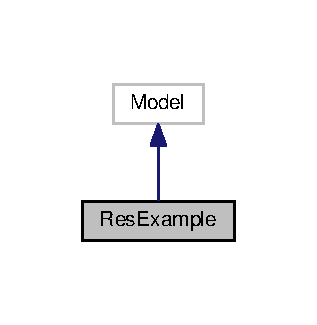
\includegraphics[width=152pt]{class_res_example__inherit__graph}
\end{center}
\end{figure}


Collaboration diagram for Res\-Example\-:
\nopagebreak
\begin{figure}[H]
\begin{center}
\leavevmode
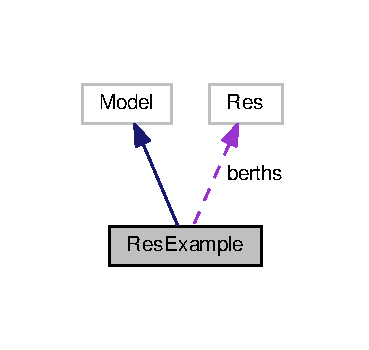
\includegraphics[width=177pt]{class_res_example__coll__graph}
\end{center}
\end{figure}
\subsection*{Public Member Functions}
\begin{DoxyCompactItemize}
\item 
\hyperlink{class_res_example_a2dcdaf535117c74d92c6fe97b255ec72}{Res\-Example} (Model owner, String name, boolean show\-In\-Report, boolean show\-Intrace)
\item 
String \hyperlink{class_res_example_a85e7862ebe831403f3da8773ba734b98}{description} ()
\item 
void \hyperlink{class_res_example_a3352131778a1ffb88f5fb1e300a1e0d5}{init} ()
\item 
void \hyperlink{class_res_example_a4855a0db355d1c1d96aa5f96ba303f37}{do\-Initial\-Schedules} ()
\end{DoxyCompactItemize}
\subsection*{Static Public Member Functions}
\begin{DoxyCompactItemize}
\item 
static void \hyperlink{class_res_example_a24f19749855594fbb1dd5e6363dfbd26}{main} (String args\mbox{[}$\,$\mbox{]})
\end{DoxyCompactItemize}
\subsection*{Protected Member Functions}
\begin{DoxyCompactItemize}
\item 
double \hyperlink{class_res_example_a7fabf49b9a1e22badd86d3d910382792}{get\-Service\-Time} ()
\item 
double \hyperlink{class_res_example_aa3f32e8d8ddbc582e6a3b7c2f890d935}{get\-Ship\-Arrival\-Time} ()
\item 
long \hyperlink{class_res_example_a0dbd04a235f2ecb12d2cb1f424cfc589}{get\-Ship\-Size} ()
\end{DoxyCompactItemize}


\subsection{Detailed Description}
This is the model class. It is the main class of a simple process-\/oriented model of the quay of a container terminal using resources to represent berths. It focuses on the allocation of berths (docking space at a quay) to incoming container ships. There are eight equal-\/sized berths on the quay in question. Every time a ship arrives it tries to allocate one, two, or three of these berths depending on its size. If there is enough space available, the container ship docks and starts unloading its freight. Otherwise, it has to wait in a queue until other ships leave the port and free the occupied berths. \begin{DoxyAuthor}{Author}
Olaf Neidhardt, Ruth Meyer 
\end{DoxyAuthor}


\subsection{Constructor \& Destructor Documentation}
\hypertarget{class_res_example_a2dcdaf535117c74d92c6fe97b255ec72}{\index{Res\-Example@{Res\-Example}!Res\-Example@{Res\-Example}}
\index{Res\-Example@{Res\-Example}!ResExample@{Res\-Example}}
\subsubsection[{Res\-Example}]{\setlength{\rightskip}{0pt plus 5cm}Res\-Example.\-Res\-Example (
\begin{DoxyParamCaption}
\item[{Model}]{owner, }
\item[{String}]{name, }
\item[{boolean}]{show\-In\-Report, }
\item[{boolean}]{show\-Intrace}
\end{DoxyParamCaption}
)}}\label{class_res_example_a2dcdaf535117c74d92c6fe97b255ec72}
\hyperlink{class_res_example}{Res\-Example} constructor.

Creates a new \hyperlink{class_res_example}{Res\-Example} model via calling the constructor of the superclass.


\begin{DoxyParams}{Parameters}
{\em owner} & the model this model is part of (set to {\ttfamily null} when there is no such model) \\
\hline
{\em model\-Name} & this model's name \\
\hline
{\em show\-In\-Report} & flag to indicate if this model shall produce output to the report file \\
\hline
{\em show\-In\-Trace} & flag to indicate if this model shall produce output to the trace file \\
\hline
\end{DoxyParams}


\subsection{Member Function Documentation}
\hypertarget{class_res_example_a85e7862ebe831403f3da8773ba734b98}{\index{Res\-Example@{Res\-Example}!description@{description}}
\index{description@{description}!ResExample@{Res\-Example}}
\subsubsection[{description}]{\setlength{\rightskip}{0pt plus 5cm}String Res\-Example.\-description (
\begin{DoxyParamCaption}
{}
\end{DoxyParamCaption}
)}}\label{class_res_example_a85e7862ebe831403f3da8773ba734b98}
returns a description of the model to be used in the report. \begin{DoxyReturn}{Returns}
model description as a string 
\end{DoxyReturn}
\hypertarget{class_res_example_a4855a0db355d1c1d96aa5f96ba303f37}{\index{Res\-Example@{Res\-Example}!do\-Initial\-Schedules@{do\-Initial\-Schedules}}
\index{do\-Initial\-Schedules@{do\-Initial\-Schedules}!ResExample@{Res\-Example}}
\subsubsection[{do\-Initial\-Schedules}]{\setlength{\rightskip}{0pt plus 5cm}void Res\-Example.\-do\-Initial\-Schedules (
\begin{DoxyParamCaption}
{}
\end{DoxyParamCaption}
)}}\label{class_res_example_a4855a0db355d1c1d96aa5f96ba303f37}
activates dynamic model components (simulation processes).

This method is used to place all events or processes on the internal event list of the simulator which are necessary to start the simulation.

In this case, only the ship generator has to be created and activated. 

Here is the call graph for this function\-:
\nopagebreak
\begin{figure}[H]
\begin{center}
\leavevmode
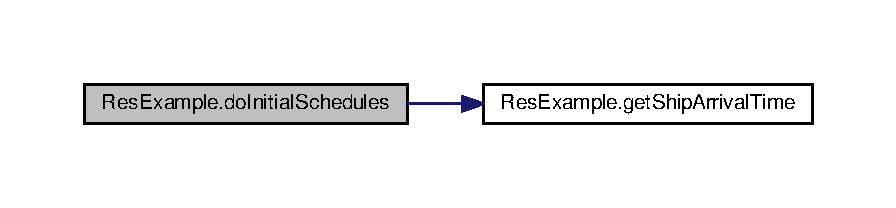
\includegraphics[width=350pt]{class_res_example_a4855a0db355d1c1d96aa5f96ba303f37_cgraph}
\end{center}
\end{figure}


\hypertarget{class_res_example_a7fabf49b9a1e22badd86d3d910382792}{\index{Res\-Example@{Res\-Example}!get\-Service\-Time@{get\-Service\-Time}}
\index{get\-Service\-Time@{get\-Service\-Time}!ResExample@{Res\-Example}}
\subsubsection[{get\-Service\-Time}]{\setlength{\rightskip}{0pt plus 5cm}double Res\-Example.\-get\-Service\-Time (
\begin{DoxyParamCaption}
{}
\end{DoxyParamCaption}
)\hspace{0.3cm}{\ttfamily [protected]}}}\label{class_res_example_a7fabf49b9a1e22badd86d3d910382792}
Returns a time span for the service time of a ship Stream is set to N\-O\-N\-N\-E\-G\-A\-T\-I\-V\-E=T\-R\-U\-E \begin{DoxyReturn}{Returns}
double 
\end{DoxyReturn}
\hypertarget{class_res_example_aa3f32e8d8ddbc582e6a3b7c2f890d935}{\index{Res\-Example@{Res\-Example}!get\-Ship\-Arrival\-Time@{get\-Ship\-Arrival\-Time}}
\index{get\-Ship\-Arrival\-Time@{get\-Ship\-Arrival\-Time}!ResExample@{Res\-Example}}
\subsubsection[{get\-Ship\-Arrival\-Time}]{\setlength{\rightskip}{0pt plus 5cm}double Res\-Example.\-get\-Ship\-Arrival\-Time (
\begin{DoxyParamCaption}
{}
\end{DoxyParamCaption}
)\hspace{0.3cm}{\ttfamily [protected]}}}\label{class_res_example_aa3f32e8d8ddbc582e6a3b7c2f890d935}
Returns a time span for the next interarrival time of a ship Stream is set to N\-O\-N\-N\-E\-G\-A\-T\-I\-V\-E=T\-R\-U\-E \begin{DoxyReturn}{Returns}
double 
\end{DoxyReturn}
\hypertarget{class_res_example_a0dbd04a235f2ecb12d2cb1f424cfc589}{\index{Res\-Example@{Res\-Example}!get\-Ship\-Size@{get\-Ship\-Size}}
\index{get\-Ship\-Size@{get\-Ship\-Size}!ResExample@{Res\-Example}}
\subsubsection[{get\-Ship\-Size}]{\setlength{\rightskip}{0pt plus 5cm}long Res\-Example.\-get\-Ship\-Size (
\begin{DoxyParamCaption}
{}
\end{DoxyParamCaption}
)\hspace{0.3cm}{\ttfamily [protected]}}}\label{class_res_example_a0dbd04a235f2ecb12d2cb1f424cfc589}
Returns the size of a ship in number of berths needed \begin{DoxyReturn}{Returns}
int 
\end{DoxyReturn}
\hypertarget{class_res_example_a3352131778a1ffb88f5fb1e300a1e0d5}{\index{Res\-Example@{Res\-Example}!init@{init}}
\index{init@{init}!ResExample@{Res\-Example}}
\subsubsection[{init}]{\setlength{\rightskip}{0pt plus 5cm}void Res\-Example.\-init (
\begin{DoxyParamCaption}
{}
\end{DoxyParamCaption}
)}}\label{class_res_example_a3352131778a1ffb88f5fb1e300a1e0d5}
initialises static model components like distributions and queues. \hypertarget{class_res_example_a24f19749855594fbb1dd5e6363dfbd26}{\index{Res\-Example@{Res\-Example}!main@{main}}
\index{main@{main}!ResExample@{Res\-Example}}
\subsubsection[{main}]{\setlength{\rightskip}{0pt plus 5cm}static void Res\-Example.\-main (
\begin{DoxyParamCaption}
\item[{String}]{args\mbox{[}$\,$\mbox{]}}
\end{DoxyParamCaption}
)\hspace{0.3cm}{\ttfamily [static]}}}\label{class_res_example_a24f19749855594fbb1dd5e6363dfbd26}
run the model 

Here is the call graph for this function\-:
\nopagebreak
\begin{figure}[H]
\begin{center}
\leavevmode
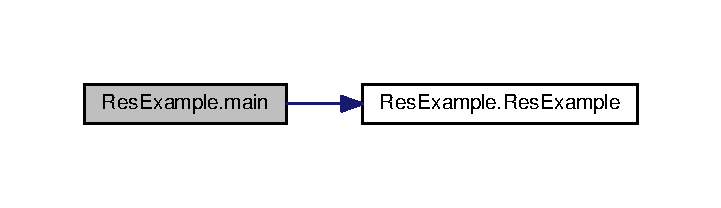
\includegraphics[width=346pt]{class_res_example_a24f19749855594fbb1dd5e6363dfbd26_cgraph}
\end{center}
\end{figure}




The documentation for this class was generated from the following file\-:\begin{DoxyCompactItemize}
\item 
src/Res\-Example.\-java\end{DoxyCompactItemize}

\hypertarget{class_ship}{\section{Ship Class Reference}
\label{class_ship}\index{Ship@{Ship}}
}


Inheritance diagram for Ship\-:
\nopagebreak
\begin{figure}[H]
\begin{center}
\leavevmode
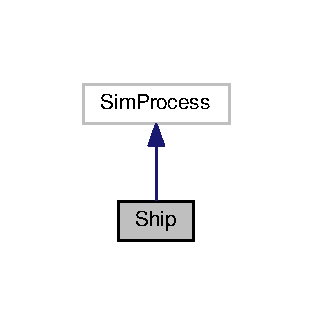
\includegraphics[width=150pt]{class_ship__inherit__graph}
\end{center}
\end{figure}


Collaboration diagram for Ship\-:
\nopagebreak
\begin{figure}[H]
\begin{center}
\leavevmode
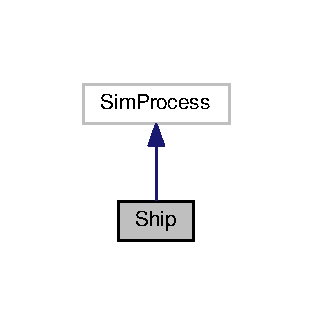
\includegraphics[width=150pt]{class_ship__coll__graph}
\end{center}
\end{figure}
\subsection*{Public Member Functions}
\begin{DoxyCompactItemize}
\item 
\hyperlink{class_ship_a8f3b6e601c7487a18699452dbdcf163c}{Ship} (Model owner, String name, boolean show\-In\-Trace)
\item 
void \hyperlink{class_ship_a553ad1866574241a0d48d80cbdb7cf21}{life\-Cycle} ()
\item 
\hypertarget{class_ship_aa5737462293bc6bca114882f482c1035}{long {\bfseries get\-Size} ()}\label{class_ship_aa5737462293bc6bca114882f482c1035}

\item 
\hypertarget{class_ship_a47761d9181d312d7153daef880566497}{void {\bfseries set\-Size} (long size)}\label{class_ship_a47761d9181d312d7153daef880566497}

\end{DoxyCompactItemize}


\subsection{Detailed Description}
This class represents a ship in the \hyperlink{class_res_example}{Res\-Example} model.

A ship arrives at the harbour and requests a number of berths according to its size. If there is enough space available, it proceeds to dock at the quay and is unloaded. Otherwise it has to wait. After service is completed, it leaves the system. \begin{DoxyAuthor}{Author}
Olaf Neidhardt, Ruth Meyer 
\end{DoxyAuthor}


\subsection{Constructor \& Destructor Documentation}
\hypertarget{class_ship_a8f3b6e601c7487a18699452dbdcf163c}{\index{Ship@{Ship}!Ship@{Ship}}
\index{Ship@{Ship}!Ship@{Ship}}
\subsubsection[{Ship}]{\setlength{\rightskip}{0pt plus 5cm}Ship.\-Ship (
\begin{DoxyParamCaption}
\item[{Model}]{owner, }
\item[{String}]{name, }
\item[{boolean}]{show\-In\-Trace}
\end{DoxyParamCaption}
)}}\label{class_ship_a8f3b6e601c7487a18699452dbdcf163c}
Constructs a new ship. 
\begin{DoxyParams}{Parameters}
{\em owner} & the model this process belongs to \\
\hline
{\em name} & this ship's name \\
\hline
{\em show\-In\-Trace} & flag to indicate if this process shall produce output for the trace \\
\hline
\end{DoxyParams}


\subsection{Member Function Documentation}
\hypertarget{class_ship_a553ad1866574241a0d48d80cbdb7cf21}{\index{Ship@{Ship}!life\-Cycle@{life\-Cycle}}
\index{life\-Cycle@{life\-Cycle}!Ship@{Ship}}
\subsubsection[{life\-Cycle}]{\setlength{\rightskip}{0pt plus 5cm}void Ship.\-life\-Cycle (
\begin{DoxyParamCaption}
{}
\end{DoxyParamCaption}
)}}\label{class_ship_a553ad1866574241a0d48d80cbdb7cf21}
Describes this ship's life cycle\-:

On arrival, the ship will request a number of berths according to its size. This will result in having the ship wait until enough space is available. It will then proceed to the quay for unloading. After service it leaves the system. 

Here is the call graph for this function\-:
\nopagebreak
\begin{figure}[H]
\begin{center}
\leavevmode
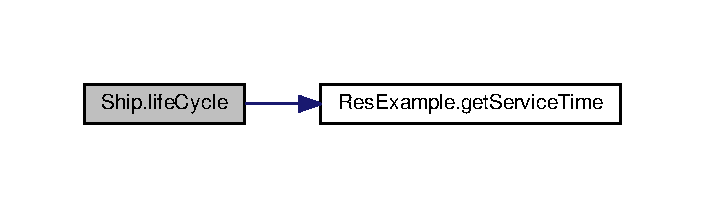
\includegraphics[width=338pt]{class_ship_a553ad1866574241a0d48d80cbdb7cf21_cgraph}
\end{center}
\end{figure}




The documentation for this class was generated from the following file\-:\begin{DoxyCompactItemize}
\item 
src/Ship.\-java\end{DoxyCompactItemize}

\hypertarget{class_ship_generator}{\section{Ship\-Generator Class Reference}
\label{class_ship_generator}\index{Ship\-Generator@{Ship\-Generator}}
}


Inheritance diagram for Ship\-Generator\-:
\nopagebreak
\begin{figure}[H]
\begin{center}
\leavevmode
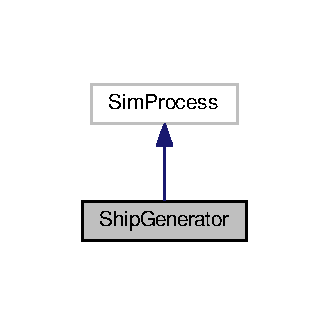
\includegraphics[width=158pt]{class_ship_generator__inherit__graph}
\end{center}
\end{figure}


Collaboration diagram for Ship\-Generator\-:
\nopagebreak
\begin{figure}[H]
\begin{center}
\leavevmode
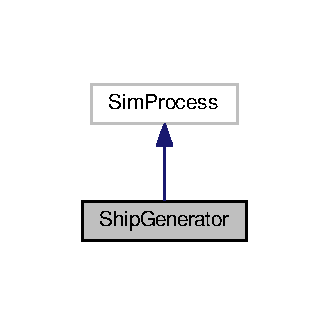
\includegraphics[width=158pt]{class_ship_generator__coll__graph}
\end{center}
\end{figure}
\subsection*{Public Member Functions}
\begin{DoxyCompactItemize}
\item 
\hyperlink{class_ship_generator_a0f5dd5eea4a965e376cdaa84109e7197}{Ship\-Generator} (Model owner, String name, boolean show\-In\-Trace)
\item 
void \hyperlink{class_ship_generator_a2a03df464499a472d8b385cfd2546f69}{life\-Cycle} ()
\end{DoxyCompactItemize}


\subsection{Detailed Description}
This class represents a process source, which continually generates ships in order to keep the simulation running.

It will create a new ship, activate it (so that it arrives at the quai) and then wait until the next ship arrival is due. \begin{DoxyAuthor}{Author}
Ruth Meyer 
\end{DoxyAuthor}


\subsection{Constructor \& Destructor Documentation}
\hypertarget{class_ship_generator_a0f5dd5eea4a965e376cdaa84109e7197}{\index{Ship\-Generator@{Ship\-Generator}!Ship\-Generator@{Ship\-Generator}}
\index{Ship\-Generator@{Ship\-Generator}!ShipGenerator@{Ship\-Generator}}
\subsubsection[{Ship\-Generator}]{\setlength{\rightskip}{0pt plus 5cm}Ship\-Generator.\-Ship\-Generator (
\begin{DoxyParamCaption}
\item[{Model}]{owner, }
\item[{String}]{name, }
\item[{boolean}]{show\-In\-Trace}
\end{DoxyParamCaption}
)}}\label{class_ship_generator_a0f5dd5eea4a965e376cdaa84109e7197}
Constructs a new ship generator process. 
\begin{DoxyParams}{Parameters}
{\em owner} & the model this ship generator belongs to \\
\hline
{\em name} & this ship generator's name \\
\hline
{\em show\-In\-Trace} & flag to indicate if this process shall produce output for the trace \\
\hline
\end{DoxyParams}


\subsection{Member Function Documentation}
\hypertarget{class_ship_generator_a2a03df464499a472d8b385cfd2546f69}{\index{Ship\-Generator@{Ship\-Generator}!life\-Cycle@{life\-Cycle}}
\index{life\-Cycle@{life\-Cycle}!ShipGenerator@{Ship\-Generator}}
\subsubsection[{life\-Cycle}]{\setlength{\rightskip}{0pt plus 5cm}void Ship\-Generator.\-life\-Cycle (
\begin{DoxyParamCaption}
{}
\end{DoxyParamCaption}
)}}\label{class_ship_generator_a2a03df464499a472d8b385cfd2546f69}
Describes this process's life cycle\-: continually generate new ships. 

Here is the call graph for this function\-:
\nopagebreak
\begin{figure}[H]
\begin{center}
\leavevmode
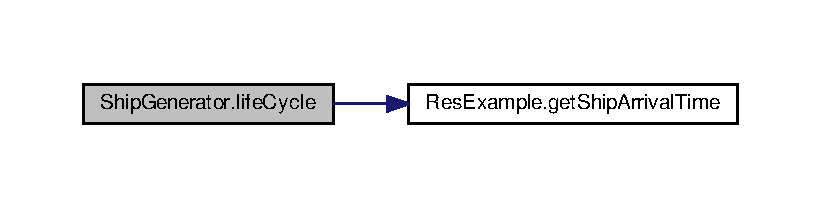
\includegraphics[width=350pt]{class_ship_generator_a2a03df464499a472d8b385cfd2546f69_cgraph}
\end{center}
\end{figure}




The documentation for this class was generated from the following file\-:\begin{DoxyCompactItemize}
\item 
src/Ship\-Generator.\-java\end{DoxyCompactItemize}

%--- End generated contents ---

% Index
\newpage
\phantomsection
\addcontentsline{toc}{part}{Index}
\printindex

\end{document}
